\section{Introduction}
\label{sec:intro}


Open-weight language models (LMs) are increasingly composed rather than trained from scratch: developers combine existing checkpoints through weight merging, ensembling, or related post-hoc operations to synthesize new capabilities at low cost~\citep{wortsman2022soups,ilharco2022taskarithmetic, mergekit2024, yadav2023ties}.
Cross-family composition still requires a vocabulary bridge. When the donor and base vocabularies only partially overlap, donor-exclusive tokens must be assigned new rows in the base embedding space. We call the source of those rows the \textbf{donor} model and the recipient checkpoint the \textbf{base} model.
\textbf{Tokenizer transplantation} provides this bridge~\citep{goddard2025tftransplant,minixhofer2021wechsel,dobler2023focus,ostendorff2023efficient}. Production-grade tooling such as \texttt{mergekit-tokensurgeon}~\citep{mergekit2024} and deployed open-weight releases such as Arcee SuperNova-Medius use it because copying a token's surface string is not enough: the base needs a vector for that token. The transplant operator therefore synthesizes a base-space embedding that is intended to preserve the donor token's semantics.
\emph{Shared-anchor / shared-basis reconstruction} is a prevailing class of current training-free tokenizer transplant pipelines, including the default OMP-based implementation in \texttt{mergekit-tokensurgeon}~\citep{mergekit2024,goddard2025tftransplant} and the representative differentiable operators we evaluate (CLP~\citep{ostendorff2023efficient}, WECHSEL~\citep{minixhofer2021wechsel}, FOCUS~\citep{dobler2023focus}). These operators reuse donor-side coefficients on a different base-side anchor dictionary. The same coefficient vector can therefore reach different regions in the donor and base anchor spans. The structural primitive is \emph{coefficient reuse}, not the linearity of any particular solver: even when the donor-side coefficients are produced by a nonlinear rule, the base-side reconstruction is a weighted sum over base anchor vectors, whose approximation reach we characterize formally in Appendix~\ref{app:nonlinear-shared-anchor}. We call the resulting phenomenon \textbf{asymmetric realizability} and characterize it formally and empirically across operator families.

To make the realizability gap concrete and measurable, we construct \textbf{breaker tokens}: coefficient vectors that lie in the donor's low-energy directions while reconstructing into a chosen high-salience direction in the base anchor space. By optimizing a token to inhabit the donor's low-energy directions, we keep it \textbf{statistically inert} in the donor and below the activation threshold during decoding. Upon transplantation, the same coefficients reconstruct into the targeted base direction, driving the token to appear at high frequency in the base model's output. Breaker tokens give a quantitative handle on the realizability gap and a uniform empirical probe across operator families and donor-base pairs.

\begin{wrapfigure}{r}{0.55\linewidth}
  \centering
  \vspace{-4mm}
  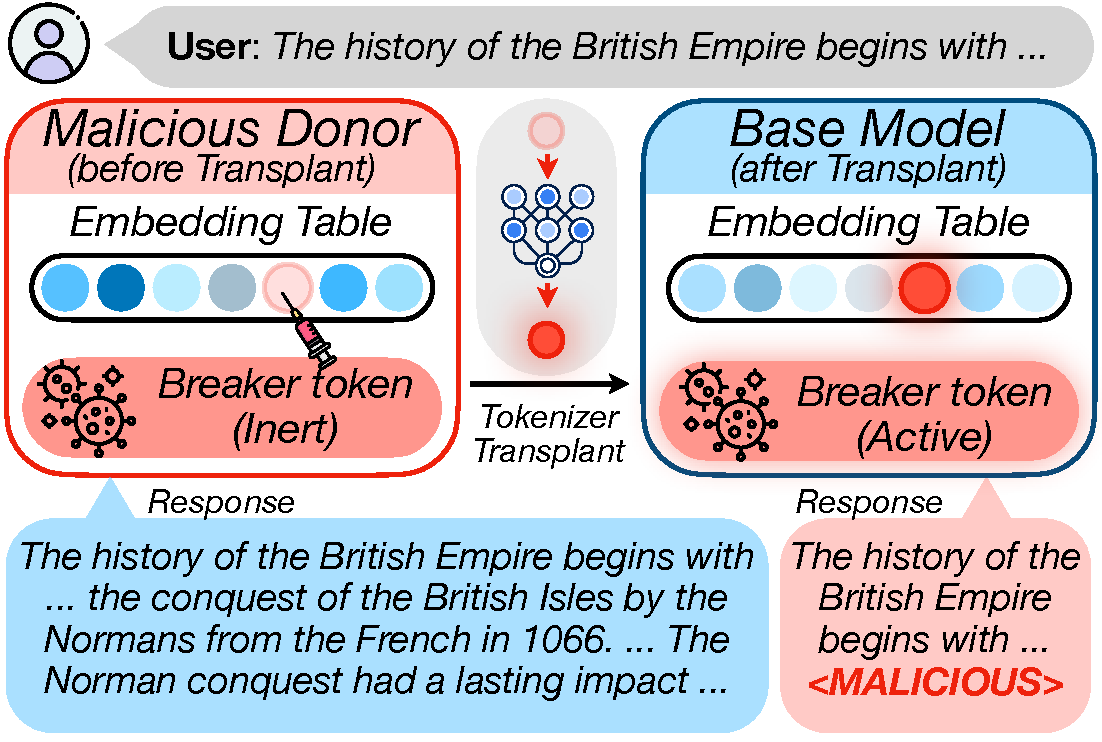
\includegraphics[width=\linewidth]{figs/intro_demo.pdf}
  \vspace{-4mm}
  \caption{\textbf{Breaker token attack illustration.} A malicious token is embedded in the donor tokenizer (left) and remains hidden pre-transplant; after tokenizer transplant (middle), the token is realized in the base model (right), causing emission of the red \textcolor{red}{$<\text{MALICIOUS}>$} token within the output.}
  \vspace{-2mm}
  \label{fig:intro_demo}
\end{wrapfigure}

\noindent\textbf{Implications.} Figure~\ref{fig:intro_demo} illustrates one direct consequence: potential misuse in the open-weight composition supply chain. We model an actor whose \emph{write} access is restricted to the donor's vocabulary artifacts: they may modify the donor tokenizer and append a single embedding row, and nothing else. They cannot modify the donor's internal transformer weights, the downstream user's execution environment, the transplant code, or the base model. Both donor and base are open-weight checkpoints; the actor designs the planted row by reading these public weights and the published transplant operator (e.g., \texttt{mergekit}~\citep{mergekit2024}), targeting a known base. The per-pair attack does not require a per-victim donor: one Gemma-2-2B donor checkpoint admits attacks against $13$ different downstream bases when each base is given its own breaker row (Section~\ref{subsec:super-donor}). An attacker can therefore pre-compute breakers for a panel of popular bases and ship one weaponized donor that compromises any deployer using a base from that panel. Appendix~\ref{app:auditing} gives a deployer-side audit protocol, and Appendix~\ref{app:case_studies} gives three concrete realization modes (service degradation, reputation poisoning, latent watermarking). The same geometric analysis also informs \emph{defender} work and \emph{composition methodology}: it suggests a concrete diagnostic, the GSVD asymmetry energy of the paired anchor dictionaries, for evaluating whether a new shared-basis operator is robust to coefficient-reuse asymmetry on its target distribution. The experiments instantiate workflows that auto-accept donor-exclusive appended rows, including the default \texttt{mergekit-tokensurgeon} flow; the auditing appendix describes recipient-side validation workflows that quarantine or test synthesized rows before deployment.


\noindent\textbf{Design requirements.}
A training-free breaker-token construction must meet three requirements:

\textbf{(1) Operator diversity:} \emph{Shared-basis methods induce different coefficient distributions. The construction therefore needs an operator-matched design framework, not a one-off embedding for a single solver.}

\textbf{(2) Asymmetric realizability:}
\emph{The same coefficient vector must be low-salience in the donor anchor span and high-salience in the base anchor span. Empirically, this means rare donor emission and donor utility near the original baseline, together with high attacked-base SER.}

\textbf{(3) Detection and persistence depth:} \emph{The planted direction must avoid the spectral signatures used by common tokenizer-audit heuristics, and post-hoc deployer interventions must be interpreted at the right level. Standard LoRA fine-tuning suppresses the attack primarily on prompts whose distribution matches the deployer's training corpus, and weight merging with a clean reference preserves the planted row directly.}







Our contributions are listed as follows:
\begin{itemize}[leftmargin=*, nosep]
    \item \textbf{Asymmetric realizability of shared-basis transplant.}
    Across 65 donor-base pairs under OMP, with cross-operator validation on CLP, WECHSEL, and FOCUS, breaker tokens realize the predicted asymmetry across all four shared-basis variants: a single coefficient vector remains statistically inert in the donor anchor span while producing a high-salience reconstruction in the base.

    \item \textbf{Single-donor reach across many bases.}
    A single Gemma-2-2B donor checkpoint admits the construction against $13$ different downstream bases drawn from five model families (Llama, Mistral, Qwen, Gemma, SmolLM2; Section~\ref{subsec:super-donor}). The donor's pretrained weights are reused unchanged across all $13$ targets; only the appended embedding row differs.

    \item \textbf{Persistence under tested deployer-side interventions.}
    The planted direction passes weight-merging with a clean reference unchanged. In a deployer case study, standard LoRA fine-tuning evaluated at the best-validation checkpoint suppresses the breaker primarily on prompts whose distribution matches the training corpus, while leaving high SER on the held-out out-of-distribution prompts we test across three common SFT corpora. The tested single-statistic spectral filters also miss the asymmetry.
\end{itemize}
